\documentclass[11pt]{standalone}
\usepackage{tikz}
\usetikzlibrary{arrows}
% Define the layers to draw the diagram
\pgfdeclarelayer{background}
\pgfdeclarelayer{foreground}
\pgfsetlayers{background,main,foreground}

% Define block styles
\tikzstyle{materia}=[draw, fill=blue!12, text width=6.0em, text centered,
  minimum height=1.5em]
% \tikzstyle{practica} = [materia, text width=8em, minimum width=10em, minimum height=3em, rounded corners,]
\tikzstyle{practica} = [materia,text width = 12em, minimum height=3em, rounded corners]
\tikzstyle{texto} = [above, text width=6em, text centered]
\tikzstyle{linepart} = [draw, thick, color=black!50, -latex', dashed]
\tikzstyle{line} = [draw, thick, color=black!50, -latex']
\tikzstyle{ur}=[draw, text centered, minimum height=0.01em]

% Define distances for bordering
\newcommand{\blockdist}{1.3}
\newcommand{\edgedist}{1.5}

\newcounter{practicaCounter}

\newcommand{\practica}[1]{\stepcounter{practicaCounter} node (p\arabic{practicaCounter}) [practica]
  {#1}}

% Draw background
\newcommand{\background}[5]{%
  \begin{pgfonlayer}{background}
    % Left-top corner of the background rectangle
    \path (#1.west |- #2.north)+(-0.5,0.5) node (a1) {};
    % Right-bottom corner of the background rectanle
    \path (#3.east |- #4.south)+(+0.5,-0.25) node (a2) {};
    % Draw the background
    \path[fill=yellow!20,rounded corners, draw=black!50, dashed]
      (a1) rectangle (a2);
    \path (a1.east |- a1.south)+(0.8,-0.3) node (u1)[texto]
      {\scriptsize\textit{Unidad #5}};
  \end{pgfonlayer}}

\newcommand{\transreceptor}[3]{%
  \path [linepart] (#1.east) -- node [above]
    {\scriptsize Transreceptor #2} (#3);}

\usepackage{bookman}
% \usepackage{times}


\begin{document}
\sffamily
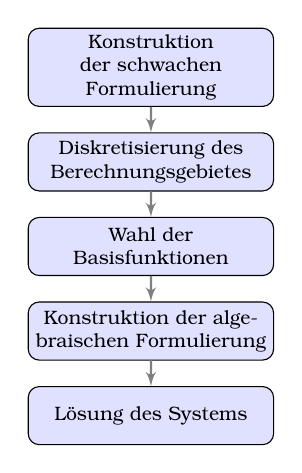
\begin{tikzpicture}[scale=0.7,transform shape]

  \path node (p1) [practica] {Konstruktion der schwachen Formulierung};
  \path (p1.south)+(0.0,-1.0) node (p2) [practica] {Diskretisierung des Berechnungsgebietes};
  \path (p2.south)+(0.0,-1.0) node (p3) [practica] {Wahl der \\ Basisfunktionen};
  \path (p3.south)+(0.0,-1.0) node (p4) [practica] {Konstruktion der algebraischen Formulierung};
  \path (p4.south)+(0.0,-1.0) node (p5) [practica] {Lösung des Systems};

  \path [line] (p1.south) -- node [above] {} (p2);
  \path [line] (p2.south) -- node [above] {} (p3);
  \path [line] (p3.south) -- node [above] {} (p4);
  \path [line] (p4.south) -- node [above] {} (p5);
\end{tikzpicture}
\end{document}
